\chapter{Training optimization} \label{training optimization}
In this chapter, the methods and settings to optimize the training process in the pipeline are shown, including but not limited to distributed training, early stopping, learning rate schedule and hyperparameter tuning.

\section{Distributed training} \label{distributed training}
In order to make full use of multiple \gls{gpu}s for training and speed up the training process, TensorFlow provides the distributed training \gls{api} to achieve parallel computing across multiple GPUs, machines or TPUs. Depending on the device, the strategy has five types, as shown in Table \ref{overview of the distributed training strategies in tensorflow}.

\begin{table}
    \centering
    \caption{Overview of the distributed training strategies in TensorFlow \cite{noauthor_distributed_nodate}}
    \label{overview of the distributed training strategies in tensorflow}
    \begin{tabular}{l|c|c|c|c|c}
        \hline
        \textbf{\makecell[l]{Training\\ API}} & \textbf{\makecell[c]{Mirrored \\ Strategy}} & \textbf{TPUStrategy} & \textbf{\makecell[c]{MultiWorker-\\ Mirrored\\ Strategy}} & \textbf{\makecell[c]{CentralStorage\\ Strategy}} & \textbf{\makecell[c]{ParameterServer\\ Strategy}} \\
        \hline
        \makecell[l]{Keras\\ Model.fit} & Supported & Supported & Supported & \makecell[c]{Experimental\\ Supported} & \makecell[c]{Experimental\\ Supported} \\
        \hline
        \makecell[l]{Custom\\ training\\ loop} & Supported & Supported & Supported & \makecell[c]{Experimental\\ Supported} & \makecell[c]{Experimental\\ Supported} \\
        \hline
        \makecell[l]{Estimator\\ API} & \makecell[c]{Limited\\ Support} & \makecell[c]{Not\\ Supported} & \makecell[c]{Limited\\ Support} & \makecell[c]{Limited\\ Support} & \makecell[c]{Limited\\ Support} \\
        \hline
    \end{tabular}
\end{table}

According to the case in our pipeline, the custom training loop is chosen and multiple GPUs with the same model in the same machine for each training are used, so the mirrored strategy is more in line with our needs. The principle is illustrated in Figure \ref{illustration of the mirrored distributed training strategy}, that is, it will divide the mini-batch data equally by the number of \glspl{gpu} into each \gls{gpu}, where each small divided data of the mini-batch is called a replica. The \gls{gpu}s contain the same model, and each \gls{gpu} uses the replica for training to update parameters, obtain loss and super-resolution range-Doppler maps. Once all GPUs have completed the training process, the obtained parameters and losses are averaged, and all super-resolution range-Doppler maps can be concatenated, then the training process of a batch of data is finished.

\begin{figure}
	\centering
	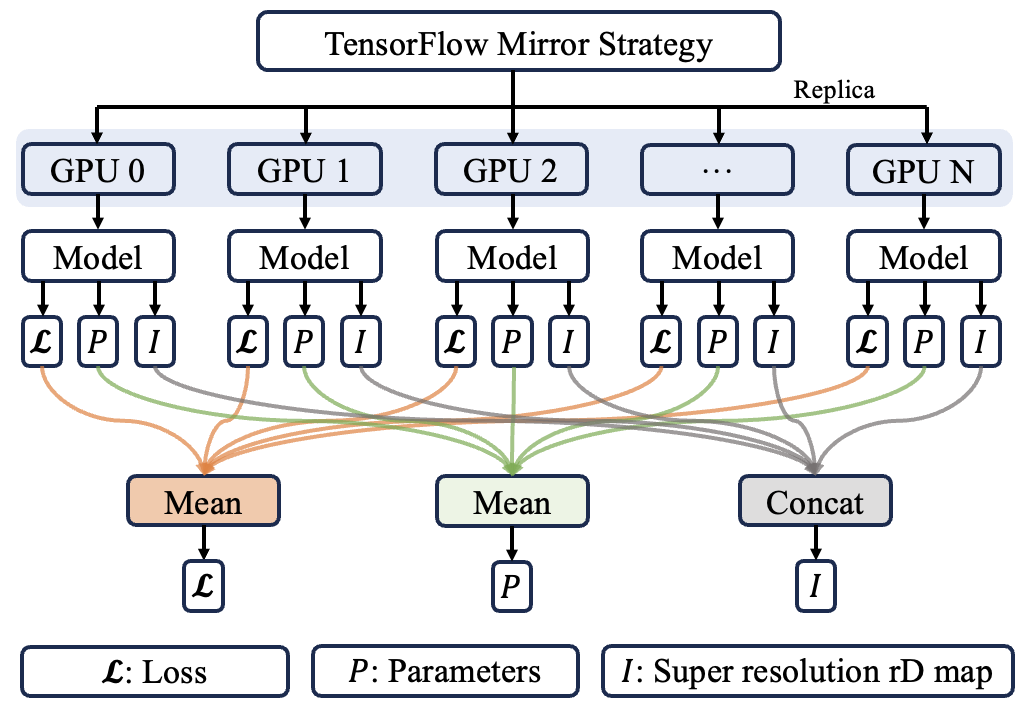
\includegraphics[scale=.65]{thesis/figures/distributed_training.png}
	\caption{Illustration of the mirrored distributed training strategy}
	\label{illustration of the mirrored distributed training strategy}
\end{figure}

Compared with the original custom training loop, the updates in the pipeline are using strategy to load the model and the optimizer, as well as set up the checkpoint. Additionally, the custom training loop should be run as a new loop within the strategy loop, so that the strategy will automatically divide the batch and average the loss and parameters. It is noted that the operation on the loss should be selected as sum by default, since the strategy will then automatically calculate the average of the sum value.

\section{Settings in the pipeline} \label{settings in the pipeline}
In this section, some settings are introduced in order to speed up the training process as well as save the checkpoints for restoring the model in the evaluation phase.

\begin{spacing}{1.5}
\textbf{\large{Early stopping}}
\end{spacing}
In the training loop, the training and validation losses are obtained after each epoch if not pretraining. Otherwise, after pretraining phase, each epoch has a validation loss. By default, the training loop is terminated if the validation loss does not decrease after 10 consecutive epochs to avoid that the training process doesn't have progress due to overfitting but occupies the resources for a long time after setting a higher number of epochs.

\begin{spacing}{1.5}
\textbf{\large{Learning rate schedule}}
\end{spacing}
In order to speed up the training process and adjust the learning rate at different training stages to help the model converge better, the learning rate schedule is used in the pipeline. According to the size of low-resolution training set as \texttt{(28353, 4, 32, 256)}. By default, after every 10,000 batches, the learning rate lowers by factor 0.96 and the initial learning rate as a hyperparameter can be determined according to the different cases. The learning rate goes as shown in Figure \ref{overview of the learning rate schedule} in the case that the number of the epochs is 200.

\begin{figure}
	\centering
	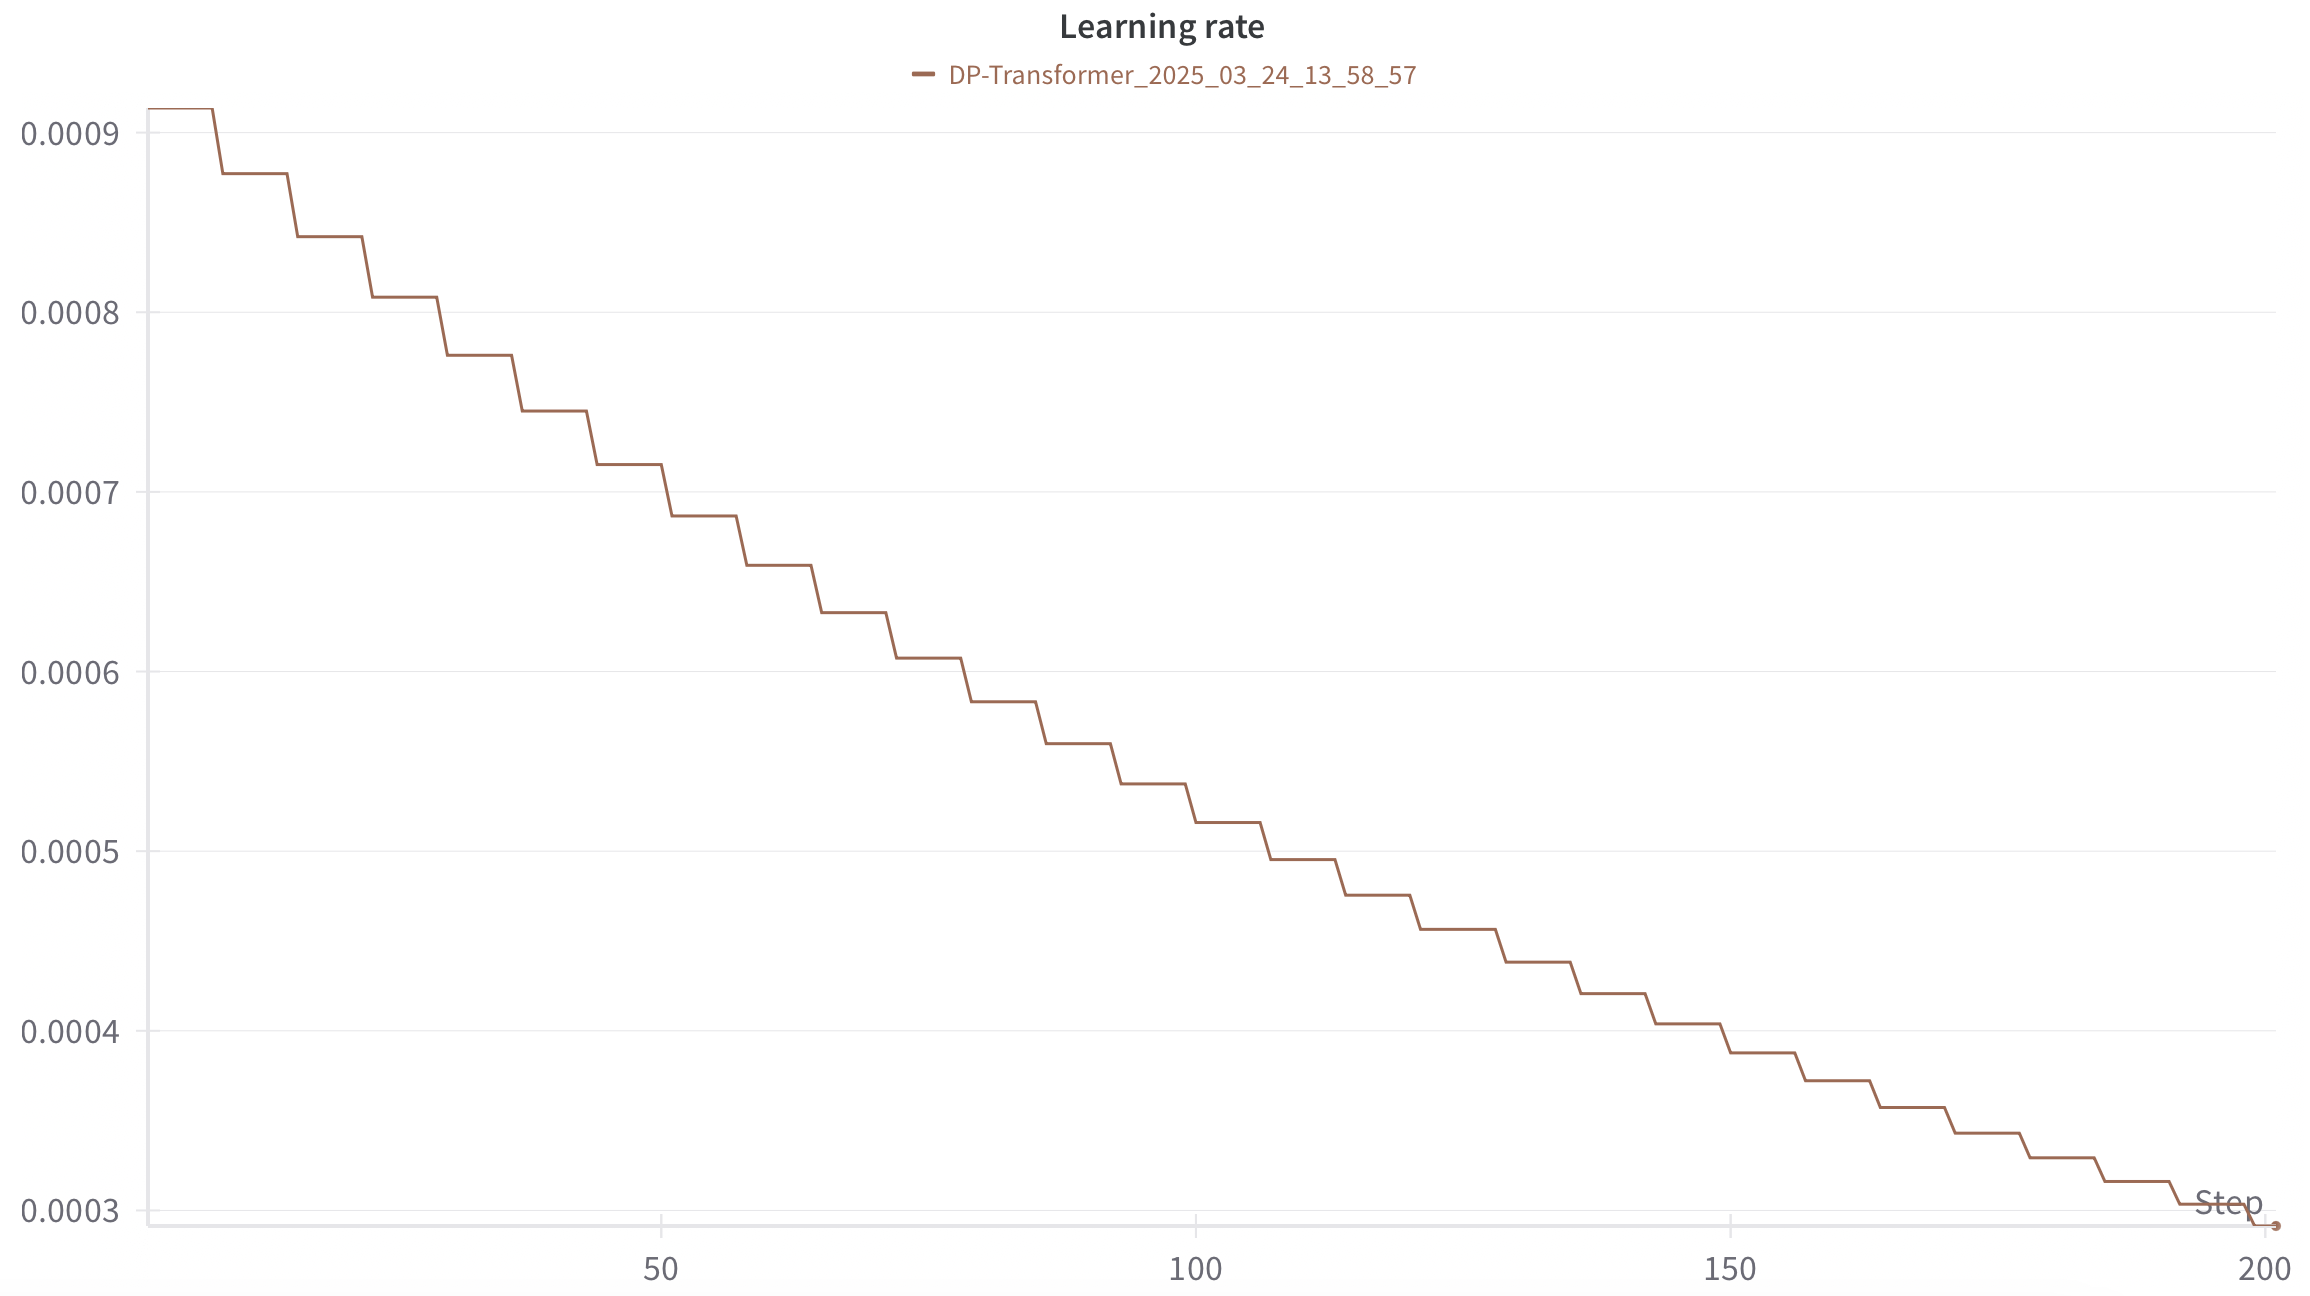
\includegraphics[scale=.3]{thesis/figures/learning_rate_schedule.png}
	\caption{Overview of the learning rate schedule in the case of 200 epochs, decay steps as 10,000, decay rate as 0.96 and initial learning rate as 9.1e-4.}
	\label{overview of the learning rate schedule}
\end{figure}

\begin{spacing}{1.5}
\textbf{\large{Checkpoint setting}}
\end{spacing}
In order to separate the training and evaluation phases and effectively prevent the interruption during the training process, the trainable parameters of the model can be saved in checkpoints. The strategy in the pipeline is by default to save the checkpoint immediately after the first epoch, and then save the current model parameters in the checkpoint as the validation loss decreases in the next epochs. To prevent storing too many checkpoints of the ealier stage, the default setting only retains the latest 5 checkpoints.

\begin{spacing}{1.5}
\textbf{\large{WandB}}
\end{spacing}
\gls{wandb} \cite{wandb_site_2025} is a tool that can be used to track, visualize, and collaborate on machine learning projects. It provides many functions, such as tracking indicators, storing data, tuning hyperparameters, and visualizing models. In our pipeline, \gls{wandb} is mainly used for recording and tuning. In the training loop, \gls{wandb} will record the low-resolution, super-resolution, and high-resolution range-Doppler map of both the training set and validation set in the last batch of each epoch, for a total of six range-Doppler maps. Meanwhile, it records the training loss, validation loss, current best validation loss, learning rate, and running time of each epoch, where Figure \ref{overview of the learning rate schedule} is recorded by \gls{wandb}. Furthermore, \gls{wandb} will automatically record some system usage, such as memory usage, power usage, etc. Additionally, in our pipeline, \gls{wandb} is also used for sweeping the hyperparameters to tune.

\begin{spacing}{1.5}
\textbf{\large{Optimizer}}
\end{spacing}
There are many choices for optimizers, among which \gls{bgd} and \gls{sgd} are the basic optimizers. Then the new methods were designed such as Momentum, which are used to speed up optimization and convergence. After that, optimizers such as \gls{adagrad} and \gls{rmsprop} were proposed, which will optimize the parameters according to the importance, namely larger updates to parameters with low importance but smaller updates to parameters with high importance, which greatly improves robustness as well. The most commonly used optimizer at present is \gls{adam}, which effectively combines the advantages of \gls{rmsprop} and Momentum and achieves better results \cite{kingma_adam_2017}.

In our pipeline, the Adam optimizer is used by default. During the tuning process, the other above-mentioned adaptive optimizers could be tested, such as \gls{rmsprop} and so on. Moreover, there are two \gls{api}s to load optimizer in TensorFlow, where the \texttt{tf.keras.optimizers.legacy} requires a higher version of TensorFlow but can provide faster speed, while the normal \texttt{tf.keras.optimizers} is suitable for lower versions, so the lower version is used by default in the server but can use the faster one in the local computer.

\begin{spacing}{1.5}
\textbf{\large{Pre-training}}
\end{spacing}
Since the training with \gls{vgg} perceptual loss and \gls{cgan} is not stable in the early epochs and in order to make sure that the optimization of the model goes to the ideal direction, we introduced the pretraining phase. As a training loss function is combined with perceptual loss, or when cGAN is used, the training processing will be only affected by the \gls{lsd} loss function in the first 50 epochs by default to ensure the stability in the early stage.


\section{Hyperparameter optimization} \label{hyperparameter optimization}
\gls{wandb} provides a sweep function that can be used to combine different hyperparameters and find the optimal solution based on the goal. In our pipeline, \gls{wandb} will record the best validation loss during training, and hence, the goal is set to minimize this value during tuning. Sweep function provides a variety of combination methods, such as grid, random, and Bayes, among which random combination of the hyperparameters is the most common method. In the pipeline, multiple specified configuration files of each model can be created to save the hyperparameters which are going to be tuned, so that the settings can be modified easily during the tuning process. For the training loop, some settings or hyperparameters can be tuned, such as the type of optimizer, learning rate, batch size, etc. In terms of the models, such as \gls{dp}-\gls{tf} Transformer model, the hyperparameters to be tuned could be the number of filters, the kernel size of encoder and decoder, as well as the number of the blocks, etc.